\documentclass[10pt,twocolumn,letterpaper]{article}

\usepackage{cvpr}
\usepackage{times}
\usepackage{epsfig}
\usepackage{graphicx}
\usepackage{amsmath}
\usepackage{amssymb}
\usepackage{tikz}

% Include other packages here, before hyperref.

% If you comment hyperref and then uncomment it, you should delete
% egpaper.aux before re-running latex.  (Or just hit 'q' on the first latex
% run, let it finish, and you should be clear).
\usepackage[breaklinks=true,bookmarks=false]{hyperref}

\cvprfinalcopy % *** Uncomment this line for the final submission

\def\cvprPaperID{****} % *** Enter the CVPR Paper ID here
\def\httilde{\mbox{\tt\raisebox{-.5ex}{\symbol{126}}}}

% Pages are numbered in submission mode, and unnumbered in camera-ready
%\ifcvprfinal\pagestyle{empty}\fi
\setcounter{page}{4321}
\begin{document}

%%%%%%%%% TITLE
\title{Articulated Motion Models for Scene Understanding}

\author{Suren Kumar\\
State University of New York at Buffalo \\
Buffalo, NY \\
{\tt\small surenkum@buffalo.edu}
% For a paper whose authors are all at the same institution,
% omit the following lines up until the closing ``}''.
% Additional authors and addresses can be added with ``\and'',
% just like the second author.
% To save space, use either the email address or home page, not both
\and
Vikas Dhiman\\
University of Michigan\\
Ann Arbor, MI\\
{\tt\small dhiman@umich.edu}
}

\maketitle
%\thispagestyle{empty}

%%%%%%%%% ABSTRACT
\begin{abstract}
We hypothesize a articulated model world view of scene understanding by representing scene as collection of objects/bodies (humans, chairs, doors, walls, floor etc.) which are connected to each other by various types of articulated joints (prismatic, revolute, static, motion along a plane etc.). Spatial structure of scene is due to the nature of these articulated joints, i.e. objects do not exhibit motions with full degree of freedom (6 for 3-dimensional world) but instead have a structure afforded by the articulated joint (door moves about a hinge). Along with this spatial structure, we hypothesize motion in world is temporally structured by finite order of motion. We use this spatio-temporal structure to represent the scene and demonstrate the proposed framework for the problem of Simultaneous localization and Area Mapping in dynamic environments.
\end{abstract}

%%%%%%%%% BODY TEXT
\section{Introduction}

Imagine a robot moving in a typical living room environment which encounters indoor objects such as doors, drawers and chairs etc. We posit that in order for the robot to understand, map or interact with such objects, the robot needs to be able to understand the articulation. Pyschophysical experiments on human motion understanding have demonstrated that human first distinguish between competing motion models (translation, rotation and expansion) and then estimate the motion conditioned on motion model \cite{NIPS2008_3458}. 

%-------------------------------------------------------------------------
\section{Motion Models in Literature}
There is significant interest in modelling motion for object tracking in computer vision literature \cite{cifuentes2012motion}. However the modelling of motion is often done in image space with simplistic models such as move left/move right which does not explain the motion of objects in physical world. Yan and Pollefeys \cite{yan2006automatic} proposed a model to detect the articulated structure of a object by using Structure from motion and then clustering trajectories to find articulation. But their approach only models revolute joint and doesn't model the temporal structure. 

There has been tremendous interest in robotics community to learn the kinematic structure such as the type of articulation from depth data \cite{sturm2010vision,katz2013interactive,katz2014interactive}. However the primary limitations of these methods is limitation of the work space. All of these methods don't model the appearance/dis-appearance of objects from the scene because they do not make any map of the world. Furthermore, these approaches are restrictive in terms of the joint models they consider which don't include joints like motion on a plane.

SLAM deals with dynamic environment in two different ways, 1) State Augmentation, 2) Outlier Rejection. State augmentation approach adds the state of the moving objects to the overall state being estimated \cite{wang2003online}. State augmentation approaches \cite{wang2003online,kundu2011realtime} assume the separation of measurement into stationary and moving objects and map is still built from static features.  On the other hand outlier rejection aims to detect and remove the objects/landmarks from the mapping and localization estimation. However, both these approaches fail to model the motion of moving features/landmarks in a robust manner which precludes the possibility of using moving landmarks for both localization and mapping.  The generic and common method used to model the motion is that of constant velocity model in 3D euclidean coordinates \cite{wang2003online}, Special Euclidean group SE(3) of transformation \cite{kundu2011realtime}. This velocity model is insufficient to model the physical reality such as motion of a door, movement of a chair on the floor etc.

The proposed approach proposes robust and physically inspired models of spatio-temporal motion which can thus be used to accurately describe the motion and hence enabling moving landmarks to be used in localization and mapping.

\section{SLAM for Dynamic World}

\section{Preliminary experiment and Results}
We test our algorithm in a simulated environment of 3 landmarks generated with each of the motion models: static, prismatic and revolute. We assume that robot egomotion is known and we use bearing and distance observations from the robot to estimate different motion models over time. In Figure~\ref{fig:results}, the landmarks are colored on basis of estimated motion model, while trajectories are drawn when a particular motion model has probability above a threshold. Our experiments show that our EKF based motion model and parameter estimation works as expected.

\begin{figure*}[t]
  \usetikzlibrary{calc}
  \centering
   \begin{tikzpicture}[imgstyle/.style={draw,thick,anchor=south west,inner sep=1pt}]
 %\path[use as bounding box, draw] (0,-1) rectangle (\imgwidth, 0.34\imgwidth);
\node[imgstyle] (img1) at (0,0) {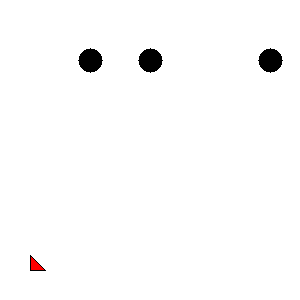
\includegraphics[width=0.32\imgwidth]{media/frame0000.png}};
\node[imgstyle] (img2) at (0.333\imgwidth,0) {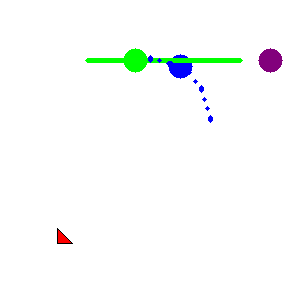
\includegraphics[width=0.32\imgwidth]
{media/frame0003.png}};
\node[imgstyle] (img3) at (0.666\imgwidth,0) {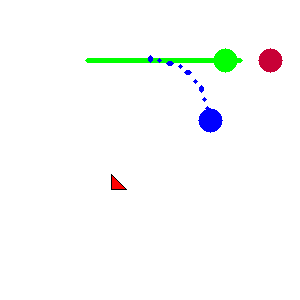
\includegraphics[width=0.32\imgwidth]{media/frame0009.png}};
\begin{scope}[x={(img1.south east)}, y={(img1.north west)}]
\node (r) at (0.3, 0.1) {Robot};
\node (lmks) at (0.7, 0.6) {Landmarks};
\end{scope}
\path ($(img1.south) + (-0.5, -0.5)$) node (ld) {Legend:};
\path 
(ld)
 ++ (1.8, 0) node [circle,fill=green] {} + (1, 0) node {Prismatic}
 ++ (3, 0) node [circle,fill=blue] {} + (1, 0) node {Revolute}
 ++ (3, 0) node [circle,fill=red] {} + (0.8, 0) node {Static}
;

 \end{tikzpicture}

  \caption{Frames at different time intervals of our simulation.
  Color of a landmark at a particular frame is the weighted sum of colors
  assigned to each motion model. The weights used are the probability of the
  landmark following that particular motion model and estimated by our algorithm. We also show the predicted trajectory of a landmark according to the estimated motion model.}
  \label{fig:results}
\end{figure*}

{\small
\bibliographystyle{ieee}
\bibliography{articulation_scene_understanding}
}

\end{document}
